\documentclass[dvipdfmx,10pt]{beamer}
%%%% Packages %%%%%
%%%%%%%%%%%%%%%%%%%%%%%%%%%%%%%%%%%%%%%%%%%%%%%%%%%%%%%%%%%%%%%%
% User-defined Macro
%%%%%%%%%%%%%%%%%%%%%%%%%%%%%%%%%%%%%%%%%%%%%%%%%%%%%%%%%%%%%%%%
\newcommand{\compress}{\itemsep0pt\parsep0pt\parskip0pt\partopsep0pt}
% \newcommand{\compress}{\itemsep1pt plus1pt\parsep0pt\parskip0pt}
% \newcommand{\code}[1]{\lstinline[basicstyle=\ttfamily]{#1}}
\newcommand{\gringo}{\textit{gringo}}
\newcommand{\clasp}{\textit{clasp}}
\newcommand{\clingo}{\textit{clingo}}
\newcommand{\teaspoon}{\textit{teaspoon}}
\newcommand{\sat}{\textsf{SAT}}
\newcommand{\unsat}{\textsf{UNSAT}}
% \newcommand{\web}[2]{\href{#1}{#2\ \raisebox{-0.15ex}{\beamergotobutton{Web}}}}
% \newcommand{\doi}[2]{\href{#1}{#2\ \raisebox{-0.15ex}{\beamergotobutton{DOI}}}}
% \newcommand{\weblink}[1]{\web{#1}{#1}}
% \newcommand{\imp}{\mathrel{\Rightarrow}}
% \newcommand{\Iff}{\mathrel{\Leftrightarrow}}
% \newcommand{\mybox}[1]{\fbox{\rule[.2cm]{0cm}{0cm}\mbox{${#1}$}}}
% \newcommand{\mycbox}[2]{\tikz[baseline]\node[fill=#1!10,anchor=base,rounded corners=2pt] () {#2};}
% \newcommand{\naf}[1]{\ensuremath{{\sim\!\!{#1}}}}
% \newcommand{\head}[1]{\ensuremath{\mathit{head}(#1)}}
% \newcommand{\body}[1]{\ensuremath{\mathit{body}(#1)}}
% \newcommand{\atom}[1]{\ensuremath{\mathit{atom}(#1)}}
% \newcommand{\poslits}[1]{\ensuremath{{#1}^+}}
% \newcommand{\neglits}[1]{\ensuremath{{#1}^-}}
% \newcommand{\pbody}[1]{\poslits{\body{#1}}}
% \newcommand{\nbody}[1]{\neglits{\body{#1}}}
% \newcommand{\Cn}[1]{\ensuremath{\mathit{Cn}(#1)}}
% \newcommand{\reduct}[2]{\ensuremath{#1^{#2}}}
% \newcommand{\OK}{\mbox{\textcolor{green}{\Pisymbol{pzd}{52}}}}
% \newcommand{\KO}{\mbox{\textcolor{red}{\Pisymbol{pzd}{56}}}}
% \newcommand{\code}[1]{\lstinline[basicstyle=\ttfamily]{#1}}
% \newcommand{\lw}[1]{\smash{\lower2.ex\hbox{#1}}}
\newcommand{\llw}[1]{\smash{\lower3.ex\hbox{#1}}}

\newenvironment{tableC}{%
  \scriptsize
  \renewcommand{\arraystretch}{0.9}
  \tabcolsep = 0.6mm
  % \begin{tabular}[t]{p{6mm}|rlr|rlr|rlr|rlr|rlr}\hline
  %   \multicolumn{1}{l|}{\llw{問題   }} &
  \begin{tabular}[t]{l|rlr|rlr|rlr|rlr|rlr}\hline
    \multicolumn{1}{l|}{\llw{問題}} &
    \multicolumn{3}{c|}{UD1} &
    \multicolumn{3}{c|}{UD2} &
    \multicolumn{3}{c|}{UD3} &
    \multicolumn{3}{c|}{UD4} &
    \multicolumn{3}{c}{UD5} \\
    & 
    \multicolumn{1}{c}{既知の} & & \multicolumn{1}{c|}{ASP} & 
    \multicolumn{1}{c}{既知の} & & \multicolumn{1}{c|}{ASP} & 
    \multicolumn{1}{c}{既知の} & & \multicolumn{1}{c|}{ASP} & 
    \multicolumn{1}{c}{既知の} & & \multicolumn{1}{c|}{ASP} & 
    \multicolumn{1}{c}{既知の} & & \multicolumn{1}{c}{ASP} \\
    & 
    ベスト & &  & 
    ベスト & &  & 
    ベスト & &  & 
    ベスト & &  & 
    ベスト & &  \\
    \hline
  }{%
    \hline
  \end{tabular}
}


\begin{document}
\title{解集合プログラミングを用いた\\クイーン支配問題の解法に関する考察}
\author{101830080 \quad 加藤 聖人}
\date{2021年度 卒業研究発表会 \\ 2022年2月18日}
\institute{番原研究室}

%
%表紙
%

\begin{frame}\frametitle{}
 \titlepage
\end{frame}

%
%支配集合問題について
%

\begin{frame}\frametitle{支配集合問題}
 \begin{block}{支配集合}
% 無向グラフ$G=(V,E)$の頂点の部分集合$S\subset V$に対して,
% 任意の頂点$u \in V\setminus S$にも辺$(u,v) \in E$が存在し,
% $v \in S$を満たすとき,$S$を$G$の\structure{支配集合}という.
無向グラフ$G=(V,E)$の頂点の部分集合$S\subset V$と,
その隣接頂点の集合との和集合が$V$と一致するとき,
$S$を$G$の\alert{\bf 支配集合}という.
\begin{itemize}
\item 支配集合の要素数を\structure{\bf サイズ}という.
\item サイズが最小の支配集合をグラフ$G$の\structure{\bf 最小支配集合}という.
\item 最小支配集合のサイズをグラフ$G$の\structure{\bf 支配数}といい,
  $\gamma(G)$で表す.
\end{itemize}
\end{block}

\begin{block}{支配集合問題}
  グラフ$G$と正の整数$k$が与えられたとき,サイズ$k$の支配集合が存在す
  るかどうかを判定する問題を\alert{\bf 支配集合問題}という.
  \begin{itemize}
  \item 支配集合問題は\structure{\bf NP完全}であることが知られている.
  \item 支配集合問題は,スケジューリング,電波塔配置問題などの問題に応
    用されている.
  \end{itemize}
 \end{block}
\end{frame}

%
%クイーン支配問題
%
\begin{frame}\frametitle{クイーン支配問題(Queen Domination Problem; QDP)}

  \begin{alertblock}{クイーン支配問題}\centering
    $n\times n$のクイーングラフ$Q_n$と正の整数$k$が与えられたとき,
    サイズ$k$の支配集合が存在するかどうかを判定する問題
 \end{alertblock}
 \vfill
 \begin{itemize}
 \item $Q_n$は$n\times n$のチェス盤について各マスを頂点とし,
   クイーンが移動できるマス同士が辺で結ばれているグラフである.
 \item $n\times n$の盤面に$k$個のクイーンを置いたとき,すべてのマスに
       1つ以上のクイーンが移動できるかどうかを判定する.
 \item 古くから研究されており,1862年に文献[Jaenisch,1862]で
   支配数$\gamma(Q_8)=5$が示されている.
 \item これまで,$1\leq n\leq 25$の支配数$\gamma(Q_n)$が求められ
   ている~\footnote{\url{https://oeis.org/A075458}}.
 \end{itemize}
\end{frame}
 
 
%
%クイーン支配問題の例
%

\begin{frame}{クイーン支配問題の例}
  \begin{exampleblock}{$Q_5$の最小支配集合}
  \begin{center}
   \scalebox{1.3}{
   \begin{tikzpicture}
 \draw[lightgray] (-1.25,-1.25)--(-1.25,1.25);
 \draw[lightgray] (-0.75,-1.25)--(-0.75,1.25);
 \draw[lightgray] (-0.25,-1.25)--(-0.25,1.25); 
 \draw[lightgray] (0.25,-1.25)--(0.25,1.25); 
 \draw[lightgray] (0.75,-1.25)--(0.75,1.25); 
 \draw[lightgray] (1.25,-1.25)--(1.25,1.25); 
 \draw[lightgray] (-1.25,-1.25)--(1.25,-1.25); 
 \draw[lightgray] (-1.25,-0.75)--(1.25,-0.75); 
 \draw[lightgray] (-1.25,-0.25)--(1.25,-0.25); 
 \draw[lightgray] (-1.25,0.25)--(1.25,0.25); 
 \draw[lightgray] (-1.25,0.75)--(1.25,0.75); 
 \draw[lightgray] (-1.25,1.25)--(1.25,1.25); 
 \draw (-1.25,1)--(1.25,1);
 \draw (-1,1.25)--(-1,-1.25);
 \draw (-1.25,1.25)--(1.25,-1.25);
 \draw (-1.25,0.75)--(-0.75,1.25);
 \draw (-1.25,-1)--(1.25,-1);
 \draw (-0.5,-1.25)--(-0.5,1.25);
 \draw (-0.25,-1.25)--(-1.25,-0.25);
 \draw (-0.75,-1.25)--(1.25,0.75);
 \draw (1,1.25)--(1,-1.25);
 \draw (-1.25,0.5)--(1.25,0.5);
 \draw (0.25,1.25)--(1.25,0.25);
\foreach \x in {-1,-0.5,0,0.5,1}
  \foreach \y in {-1,-0.5,0,0.5,1} 
  \fill (\x,\y) circle (0.03);
  \matrix[matrix of nodes,nodes={inner sep=0pt,text width=0.5cm,
align=center,minimum height=0.43cm}]{
 \symqueen & \quad & \quad & \quad & \quad \\
 \quad & \quad & \quad & \quad & \symqueen \\
 \quad & \quad & \quad & \quad & \quad \\
 \quad & \quad & \quad & \quad & \quad \\
 \quad & \symqueen & \quad & \quad & \quad \\};
\end{tikzpicture}
 

   }
  \end{center}
 \end{exampleblock}
 \vfill
 \begin{itemize}
  \item 3個のクイーンを置いたとき,すべてのマスに1つ以上のクイーンが移動可能である.
  \item 2個以下の場合,すべてのマスにクイーンが移動することは不可能である.
  \item したがって,支配数は$\gamma(Q_{5})=3$となる.
 \end{itemize}
\end{frame}



%
%ASPについて
%

\begin{frame}\frametitle{解集合プログラミング(Answer Set Programming; ASP)}
  \begin{block}{}\centering
    ASP は論理プログラミングから派生した宣言的プログラミングパラダイム
    の一種である.
  \end{block}
  \vfill
  \begin{itemize}
  \item \structure{ASP言語}は一階論理に基づいた知識表現言語の一種である.
%  \item \structure{論理プログラム}は,ASP のルールの有限集合である.
  \item \structure{ASPシステム}は論理プログラムから
	安定モデル意味論[Gelfond and Lifschitz '88]に基づく
	解集合を計算するシステムである.
  \item 近年ではSAT技術を応用した高速ASPシステムが実現され,
	システム検証,プランニング,システム生物学など様々な
	分野への応用が拡大している.
 \end{itemize}
 \begin{alertblock}{支配集合問題に対してASPを用いる利点}
  \begin{itemize}
   \item ASP言語の高い表現力を活かし,支配集合問題の制約を簡潔に記述可能.
   \item 拡張性が高く,様々な定式化を簡単に試すことができる.
   \item 遷移問題への拡張も容易.
     % \item 個数制約を用いて,部分和を表す制約を簡潔に記述可能.
   % \item 高速な解列挙が可能.
  \end{itemize}
 \end{alertblock}
\end{frame}
 
%
%研究目的と研究内容
%

\begin{frame}\frametitle{研究目的}
 \begin{alertblock}{研究目的}\centering
  ASP技術を活用し,支配集合問題を効率よく解くソルバーの実現.
 \end{alertblock}

 \begin{itemize}
 \item 本研究ではクイーン支配問題を対象とする.
 \item SAT型制約ソルバーを用いた既存研究~[山本,2021]で提案された制約モ
   デルを応用する.
 \end{itemize}

 \begin{block}{研究内容}
  \begin{enumerate}
   \item クイーン支配問題を解く3種類のASP符号化を考案した.
     \begin{itemize}
     \item 基本符号化
     \item 改良符号化
     \item 部分和符号化
     \end{itemize}
   \item クイーン支配問題 ($Q_{n}: 1\leq n\leq 20$) を用いた評価実験を行った.
  \end{enumerate}
 \end{block}
\end{frame}

%
%符号化3つ
%

\begin{frame}{考案したASP符号化}

  \begin{block}{クイーン支配問題の制約}
    \begin{itemize}
    \item チェスの盤面上に$k$個のクイーンが配置される(個数制約)
    \item どのマスにも,1つ以上のクイーンが移動できる(移動制約)
    \end{itemize}
  \end{block}

  \begin{enumerate}
  \item \structure{\bf 基本符号化}
    \begin{itemize}
    \item マス$(i,j)$に対して,クイーンの有無を表すアトム$q(i,j)$を導
      入する.
    \item $q(i,j)$を用いて,個数制約を表現する.
    \item マスごとに移動制約を満たすかどうかチェックする.
    \end{itemize}
 \item \structure{\bf 改良符号化}
   \begin{itemize}
    \item 個数制約は基本符号化と同じ.
    \item 各行,各列,各対角線ごとにクイーンの有無を表す補助アトムを導入し,
      移動制約を満たすかどうかチェックする.      
   \end{itemize}
 \item \alert{\bf 部分和符号化}
   \begin{itemize}
   \item 各行,各列,各対角線ごとに
     クイーンの個数を表す補助アトムを導入し,
     個数制約と移動制約を表現する.
   \end{itemize}
 \end{enumerate}
\end{frame}


%
% 部分和符号化
%

\begin{frame}\frametitle{部分和符号化の特徴: 行方向の推論}
  \begin{itemize}
   % \item \structure{\bf アトム$q(i,j)$:} \quad $q(i,j)=\{0,1\}$
   % 	 \begin{itemize}
   % 	  \item アトム$q(i,j)$が1のとき,マス$(i,j)$にクイーン
   % 		が配置される.
   % 	 \end{itemize}
   \item \structure{\bf 補助アトム$r_i$:}\quad $r_{i}=\sum\limits_{j=1}^{n} 
	      q(i,j) \qquad (1 \leq i \leq n)$ 
	 \begin{itemize}
	  \item 行$i$上のクイーンの個数を$r_i$とする.
	 \end{itemize}
   \item \structure{\bf 個数制約:}\quad $\sum\limits_{i=1}^{n}r_{i} = k$
	 \begin{itemize}
	  \item 行ごとのクイーンの合計は盤面全体の数に一致する.
	 \end{itemize}
   \item \structure{\bf 移動制約:}\quad $(r_{i}>0 \vee c_{j}>0 \vee 
	 u_{i+j}>0 \vee d_{i-j} > 0) =1  \quad (1\leq i,j \leq n)$ 
	 \begin{itemize}
	  \item マス$(i,j)$にクイーンが1つ以上移動できる.
	  \item $c_{j}$, $u_{i+j}$, $d_{i-j}$は,
		列方向,対角線方向の補助アトム
	 \end{itemize}
  \end{itemize}
 \begin{exampleblock}{例:$Q_{5},k=3$}
  \begin{columns}
   \begin{column}{0.45\textwidth}
    \centering
    \scalebox{1}{
    %%%%%%%%%%%%%%%%%%%%%%%%%%%%%%%%%%%%%%%%%%%%%%%%%%
% 実行例(t=0) (第6章で使う)
%%%%%%%%%%%%%%%%%%%%%%%%%%%%%%%%%%%%%%%%%%%%%%%%%%

\begin{tikzpicture}[scale=0.6]

  % 設定
  \tikzset{node/.style={circle,draw=black}}
 
  \definecolor{col_r}{RGB}{230,0,18}
  %\definecolor{col_b}{RGB}{0,104,183}
  \definecolor{col_b}{RGB}{51,51,179}
  \definecolor{col_y}{RGB}{255,251,0}
  \definecolor{col_g}{RGB}{0,96,0}
 
  % 補助線
  % \draw [help lines,blue] (0,0) grid (20,6);
 
  % node %
  \node[node, fill=col_y!70] (node1){\textbf{1}};
  \node[node, fill=col_b!70, right=of node1] (node2){\textbf{2}};
  \node[node, fill=col_y!70, below=of node1] (node3){\textbf{3}};
  \node[node, fill=col_g!70, below=of node2] (node4){\textbf{4}};
 
  \foreach \u / \v in {node1/node2, node2/node3, node2/node4, node3/node4}
  \draw (\u) -- (\v);
 \end{tikzpicture}
 
 %%%%%%%%%%%%%%%%%%%%%%%%%%%%%%%%%%%%%%%%%%%%%%%%%%%%%%%%%%
 %%% Local Variables:
 %%% mode: japanese-latex
 %%% TeX-master: paper.tex
 %%% End:
 
    }
   \end{column}
   \begin{column}{0.45\textwidth}
    \centering
    \scalebox{1}{
    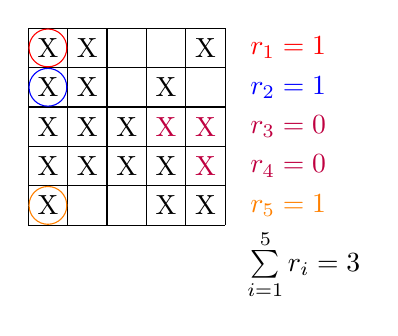
\begin{tikzpicture}
 \draw (0,0)--(2.5,0);
 \draw (0,0.5)--(2.5,0.5);
 \draw (0,1.0)--(2.5,1.0);
 \draw (0,1.5)--(2.5,1.5);
 \draw (0,2.0)--(2.5,2.0);
 \draw (0,2.5)--(2.5,2.5);
 \draw (0,0)--(0,2.5);
 \draw (0.5,0)--(0.5,2.5);
 \draw (1.0,0)--(1.0,2.5);
 \draw (1.5,0)--(1.5,2.5);
 \draw (2.0,0)--(2.0,2.5);
 \draw (2.5,0)--(2.5,2.5);
 \node (X) at (0.25,0.25) {X};
 \draw [orange] (0.25,0.25) circle[radius = 0.24];
 \node (X) at (0.25,0.75) {X};
 \node (X) at (0.25,1.25) {X};
 \node (X) at (0.25,1.75) {X};
 \draw [blue] (0.25,1.75) circle[radius = 0.24];
 \node (X) at (0.25,2.25) {X};
 \draw [red] (0.25,2.25) circle[radius = 0.24];
 \node (X) at (0.75,2.25) {X};
 \node (X) at (0.75,0.75) {X};
 \node (X) at (0.75,1.25) {X};
 \node (X) at (0.75,1.75) {X};
 \node (X) at (1.25,0.75) {X};
 \node (X) at (1.25,1.25) {X};
 \node (X) at (1.75,0.25) {X};
 \node (X) at (1.75,0.75) {X};
 \node (X) at (1.75,1.25) {\color{purple}X};
 \node (X) at (1.75,1.75) {X};
 \node (X) at (2.25,0.25) {X};
 \node (X) at (2.25,0.75) {\color{purple}X};
 \node (X) at (2.25,1.25) {\color{purple}X};
 \node (X) at (2.25,2.25) {X};
 \node (A) at (3.30,2.25) {\color{red}$r_{1} = 1$};
 \node (B) at (3.30,1.75) {\color{blue}$r_{2} = 1$};
 \node (M) at (3.30,1.25) {\color{purple}$r_{3} = 0$};
 \node (M) at (3.30,0.75) {\color{purple}$r_{4} = 0$};
 \node (C) at (3.30,0.25) {\color{orange}$r_{5} = 1$};
 \node (D) at (3.50,-0.50) {$\sum\limits_{i=1}^{5}r_{i}=3$};
\end{tikzpicture}
    }
   \end{column}
  \end{columns}
  \begin{itemize}
   \item 左の状態から,個数制約と移動制約により右の状態を推論できる.
  \end{itemize}
 \end{exampleblock}
\end{frame}


%
% 実験概要
%
\begin{frame}\frametitle{実験概要}
  \begin{block}{}\centering
    考案したASP符号化の有効性を評価するために実験を行った.    
  \end{block}
  \vfill
  \begin{itemize}
  \item \structure{\bf 比較するASP符号化}
    \begin{itemize}
    \item 基本符号化
    \item 改良符号化
    \item 部分和符号化
    \end{itemize}
  \item \structure{\bf クイーン支配問題}
    \begin{itemize}
    \item クイーングラフ $Q_{n}$ \quad ($1 \leq n \leq 20)$
    \item サイズ$k$には,充足可能(\textsf{SAT})なケースとし
      て既知の支配数$k=\gamma(Q_{n})$,
      充足不能(\textsf{UNSAT})なケースとして$k=\gamma(Q_{n})-1$ を使用.
    \end{itemize}
  \item \structure{\bf ASP システム:} \textit{clingo-5.5.0}
  \item \structure{\bf 制限CPU時間:} 3600秒 / 1問
  \item \structure{\bf 実験環境:} Mac mini, 3.2GHz 6コア Intel Core i7, 64GBメモリ
  \end{itemize}
\end{frame}


%
%実験結果(基本1,改良1,部分和2)
%

\begin{frame}\frametitle{実験結果: 求解に要した CPU 時間 (秒)}

 \begin{columns}
  \begin{column}{0.50\textwidth}
   \begin{table}[htbp]
     \caption{$k=\gamma(Q_{n})$ (\textsf{SAT})}
     \scalebox{0.7}{
     \centering 
 \begin{tabular}{c|c|r|r|r} %\hline
  $n$ & $k$ & 基本 & 改良 & 部分和 \\ \hline
  10 & 5 & 14.400 & 21.232 & 3.005 \\
  11 & 5 & 54.674 & 123.488 & 32.540 \\
  12 & 6 & T.O. & 56.468 & 2.147 \\
  13 & 7 & T.O. & 1281.823 & 22.412 \\  
  14 & 8 & 2797.041 & 772.276 & 10.044 \\   
  15 & 9 & T.O. & T.O. & 275.683 \\  
  16 & 9 & T.O. & T.O. & \alert{\textbf{734.878}} \\
  17 & 9 & T.O. & T.O. & T.O. \\
  18 & 9 & T.O. & T.O. & T.O. \\
  19 & 10 & T.O. & T.O. & T.O. \\
  20 & 11 & T.O. & T.O. & T.O. \\ %\hline
 \end{tabular}}
   \end{table}
  \end{column}
  \begin{column}{0.50\textwidth}
   \begin{table}[htbp]
     \caption{$k=\gamma(Q_{n})-1$ (\textsf{UNSAT})}
    \scalebox{0.7}{
     \centering 
 \begin{tabular}{c|c|r|r|r} %\hline
  $n$ & $k$ & 基本 & 改良 & 部分和 \\ \hline
  10 & 4 & 10.280 & 8.929 & 2.612 \\
  11 & 4 & 28.184 & 24.537 & 3.427 \\
  12 & 5 & 2706.092 & 2673.241 & \alert{\textbf{337.127}} \\
  13 & 6 & T.O. & T.O. & T.O. \\  
  14 & 7 & T.O. & T.O. & T.O. \\   
  15 & 8 & T.O. & T.O. & T.O. \\  
  16 & 8 & T.O. & T.O. & T.O. \\
  17 & 8 & T.O. & T.O. & T.O. \\
  18 & 8 & T.O. & T.O. & T.O. \\
  19 & 9 & T.O. & T.O. & T.O. \\
  20 & 10 & T.O. & T.O. & T.O. \\ %\hline
 \end{tabular}}
   \end{table}
  \end{column}
 \end{columns} 
 \begin{itemize}
 \item 充足可能(\textsf{SAT})の問題では,部分和符号化が$n=16$まで解き,
   その優位性を確認できた.
 \item 充足不能(\textsf{UNSAT})の問題では,解けた問題数に差はなかったが,
   判定の要したCPU時間は部分和符号化が最も短かった.
 \end{itemize}
\end{frame}

%
%まとめと今後の課題
%

\begin{frame}\frametitle{まとめ}

  \begin{block}{}\centering
    ASP を用いたクイーン支配問題の解法について述べた.
  \end{block}
  \vfill
  \begin{enumerate}
  \item クイーン支配問題を解く3種類のASP符号化を考案した.
    \begin{itemize}
    \item ASPの表現力を活かして,クイーン支配問題を簡潔に記述できるこ
      とを確認した.
    \end{itemize}
  \item クイーン支配問題 ($Q_{n}: 1\leq n\leq 20$) を用いた評価実験を行った.
    \begin{itemize}
    \item 充足可能(\textsf{SAT})の問題について,
      部分和符号化が$n=16$まで解き,その優位性を確認できた.
    \end{itemize}
  \end{enumerate}
  \vfill
  \begin{block}{今後の課題}
    \begin{itemize}
    \item 支配集合問題を解くASP符号化の改良
      \begin{itemize}
      \item 現時点では,SAT型制約ソルバーを用いた既存研究~[山本,2021]
        と比較して性能面で劣っている.
      \end{itemize}
    \item 遷移問題への拡張
    \end{itemize}
  \end{block}
\end{frame}

%
%付録
%

%%%% 補助スライド

\begin{frame}{~}
 \centering
 - 補足用 -
\end{frame} 

\begin{frame}{補足 : スマートグリッド}
 \begin{itemize}
  \item \structure{スマートグリッド}とは,電力の供給側,需要側において双方向の
		やり取りを可能にする次世代の\structure{賢い}電力網である.
  \item 従来と違い,通信技術の発達により,使用状況などを
		リアルタイムに把握することが可能となった.
  \item その時に応じた最適な配電網を構成し,制御するといったことが考えられている.
		\begin{itemize}
		 \item 電力需要の変化による,配電ロスの少ない構成.
		 \item 自然エネルギーによる発電量の変動を補う構成.
		\end{itemize}
  \item ASP言語の表現力や拡張性が,こうした条件の追加に活用できる可能性がある.
 \end{itemize}
\end{frame}

%%%%%%%%%%%%%%%%%%%%%%%%%%%%%%%%%%%%%%%%%%%%%%%%%%
%% 電気制約
%%%%%%%%%%%%%%%%%%%%%%%%%%%%%%%%%%%%%%%%%%%%%%%%%%
\begin{frame}{補足 : 電気制約}
 \begin{itemize}
  \item \alert{電気制約}は,送電する電流$\cdot$電圧の適正範囲を保証する制約.
  \begin{itemize}
   \item 供給経路の各区間で許容電流を超えない.
   \item 電気抵抗による電圧降下が許容範囲を超えない.
   \item etc.
  \end{itemize}
  \item 電流と電圧が影響し合う\structure{実数ドメイン上の制約}によって表される.
		% \begin{itemize}
		%  		 \item 送電システム上の条件など.
		% \end{itemize}
  \item 実数ドメイン上の制約は,純粋なASPのみで扱うのは\alert{困難}.
		\begin{itemize}
		 \item 緩和問題として,変電所から供給できる家庭の数に上限をつける.
		 \item ASPMT技術により,ASPで得られた解について,
			   背景理論ソルバーと連携して実数ドメイン上の制約を調べる.
		\end{itemize}
 \end{itemize}
\end{frame}


%%%%%%%%%%%%%%%%%%%%%%%%%%%%%%%%%%%%%%%%%%%%%%%%%%
%% 基礎化
%%%%%%%%%%%%%%%%%%%%%%%%%%%%%%%%%%%%%%%%%%%%%%%%%%
\begin{frame}{補足 : ASPシステム}
 
 \vspace{-0.5cm}

 \begin{figure}[htbp]
  \centering
  %%%%%%%%%%%%%%%%%%%%%%%%%%%%%%%%%%%%%%%%%%%%%%%%%%
%% 基礎化の流れの図
%%%%%%%%%%%%%%%%%%%%%%%%%%%%%%%%%%%%%%%%%%%%%%%%%%
\begin{tikzpicture}

 \definecolor{edge}{RGB}{38,38,134}
 \definecolor{node}{RGB}{220,220,249}

 \definecolor{alert_edge}{RGB}{191,0,0}
 \definecolor{alert_node}{RGB}{249,200,200}

 \definecolor{ex_edge}{RGB}{0,96,0}
 \definecolor{ex_node}{RGB}{230,239,230}

 \def\nodespace{2.4cm}

 \tikzset{block/.style={rectangle, thick, draw=edge, fill=node, text width=3cm, 
 text centered, rounded corners, text width=2cm, minimum height=1.5cm}};

 \tikzset{alertblock/.style={rectangle, thick, draw=alert_edge, fill=alert_node, 
 text width=3cm, text centered, rounded corners, text width=1.5cm, minimum height=1.2cm}};

 \node[block](ikkai){一階ASP\\プログラム};

 \node[rectangle,rounded corners, thick, draw=ex_edge, fill=ex_node, 
 right=0.22*\nodespace of ikkai, minimum width=6cm, minimum height=3cm, 
 text centered, label=ASPシステム](sys){};

 \node[block, right=\nodespace of ikkai](meidai){命題ASP\\プログラム};
 \node[block, right=\nodespace of meidai](ASP){解集合};

 \node[right=0.6*\nodespace of ikkai, text width=1.5cm, 
 text centered, text=red, anchor=south](){基礎化\\ソルバー};
 \node[right=0.4*\nodespace of meidai, text width=1.5cm, 
 text centered, text=red, anchor=south](){解集合\\ソルバー};

 
 \foreach \u / \v / \n in {ikkai/meidai,meidai/ASP}
 \draw [thick,->] (\u) to (\v);

\end{tikzpicture}
 \end{figure}

 \vspace{-0.5cm}

 \begin{exampleblock}{}
  \begin{enumerate}
   \item 一階ASPプログラムを基礎化ソルバーによって,
		 命題ASPプログラムに\alert{基礎化}する.
   \item 命題ASPプログラムについて,SAT技術を応用した解集合ソルバーが解集合を探索する.
  \end{enumerate}
 \end{exampleblock}

\end{frame}


%%%%%%%%%%%%%%%%%%%%%%%%%%%%%%%%%%%%%%%%%%%%%%%%%%
%% ASPのコード
%%%%%%%%%%%%%%%%%%%%%%%%%%%%%%%%%%%%%%%%%%%%%%%%%%
\begin{frame}[fragile]{補足 : 基本符号化のASPプログラム}
 \begin{exampleblock}{}
  \begin{center}
   %%%%%%%%%%%%%%%%%%%%%%%%%%%%%%%%%
   \lstinputlisting[numbers=left,%
   basicstyle=\ttfamily\tiny]{code/srf1.lp}
   %%%%%%%%%%%%%%%%%%%%%%%%%%%%%%%%% 
  \end{center}
 \end{exampleblock}
\end{frame}

\begin{frame}[fragile]{補足 : 改良符号化のASPプログラム}

 \begin{exampleblock}{}
  \begin{center}
   %%%%%%%%%%%%%%%%%%%%%%%%%%%%%%%%%
   \lstinputlisting[numbers=left,%
   basicstyle=\ttfamily\tiny]{code/srf2.lp}
   %%%%%%%%%%%%%%%%%%%%%%%%%%%%%%%%% 
  \end{center}
 \end{exampleblock}

\end{frame}



\end{document}
%%% Local Variables:
%%% mode: japanese-latex
%%% TeX-master: t
%%% End:
